\documentclass[11pt,a4paper]{article}
\usepackage[utf8]{inputenc}
\usepackage[T1]{fontenc}
\usepackage{lmodern}
\usepackage[a4paper,margin=2cm,bottom=2.5cm]{geometry}
\usepackage{graphicx}
\usepackage[export]{adjustbox}
\usepackage{float}
\usepackage{xcolor}
\usepackage{listings}
\usepackage{upquote}
\usepackage{enumitem}
\usepackage{fancyhdr}
\usepackage{xurl}
\usepackage[colorlinks=true,linkcolor=kulblue,urlcolor=kulblue]{hyperref}

\definecolor{kulblue}{RGB}{29, 141, 176}
\definecolor{codegreen}{rgb}{0,0.5,0}
\definecolor{codegray}{rgb}{0.5,0.5,0.5}
\definecolor{codepurple}{rgb}{0.58,0,0.82}
\definecolor{backcolour}{rgb}{0.95,0.95,0.97}

\lstdefinelanguage{CUDA}[]{C++}{
  morekeywords={__global__,__device__,__host__,__shared__,dim3,
    threadIdx,blockIdx,blockDim,gridDim,warpSize,
    cudaMallocManaged,cudaMalloc,cudaMemcpy,cudaFree,cudaDeviceSynchronize,
    cudaMemcpyHostToDevice,cudaMemcpyDeviceToHost,cudaGetLastError,cudaGetErrorString,
    cudaEvent_t,cudaEventCreate,cudaEventRecord,cudaEventSynchronize,cudaEventElapsedTime},
}

\lstdefinestyle{gca}{
  backgroundcolor=\color{backcolour},
  commentstyle=\color{codegreen},
  keywordstyle=\color{magenta}\bfseries,
  stringstyle=\color{codepurple},
  numberstyle=\tiny\color{codegray},
  basicstyle=\ttfamily\scriptsize,
  columns=fullflexible,
  breaklines=true,
  breakatwhitespace=false,
  postbreak=\mbox{\textcolor{codegray}{$\hookrightarrow$}\space},
  keepspaces=true,
  numbers=left,
  numbersep=6pt,
  showstringspaces=false,
  upquote=true,
  tabsize=4,
  frame=single,
  rulecolor=\color{backcolour},
  xleftmargin=1.5em,
  framexleftmargin=1.5em,
  literate={—}{{---}}1 {×}{{$\times$}}1 {’}{{'}}1,
}
\lstset{style=gca}

\setlength{\parindent}{0pt}
\setlength{\parskip}{0.6em}

\pagestyle{fancy}
\fancyhf{}
\fancyhead[L]{\small GCA -- Session 01}
\fancyhead[R]{\small Geavanceerde Computerarchitectuur}
\fancyfoot[L]{\small 12-11-2026}
\fancyfoot[C]{\small \thepage}
\fancyfoot[R]{\IfFileExists{figure/KULEUVEN_GENT_RGB_LOGO.png}{\includegraphics[width=2cm]{figure/KULEUVEN_GENT_RGB_LOGO.png}}{}}
\renewcommand{\headrulewidth}{0.4pt}

\title{\textbf{GCA -- Session 01}\\[2mm]\large Geavanceerde Computerarchitectuur}
\author{Joris Putteneers\\\href{mailto:joris.putteneers@kuleuven.be}{\texttt{joris.putteneers@kuleuven.be}}}
\date{12-11-2026 \quad (academic year 2026/2027)}

\begin{document}
\maketitle
\thispagestyle{fancy}
\tableofcontents
\newpage

%=====================================================================
\section{Introduction}

\subsection{Goals, learning outcomes, and expectations}

The goal of this course is to introduce students to the fundamentals of general purpose GPU programming. We shall dive into the concepts of parallel multi-thread processing, learning how to leverage the large number of GPU cores and how to efficiently use the device's memory. Among others, concepts such as atomic operation, synchronous multi-threading, and dynamic parallelism are explored during the course. In addition to guided exercises, the students will partake in a short project, tackling a research or programming challenge of their liking using the newly acquired knowledge. By the end, the students are foreseen to have the necessary understanding of GPUs and parallel programming that will allow them to utilize GPUs in their future work. Throughout the course NVIDIA GPUs and C++ are employed (CUDA API).
\begin{figure}[H]
\centering
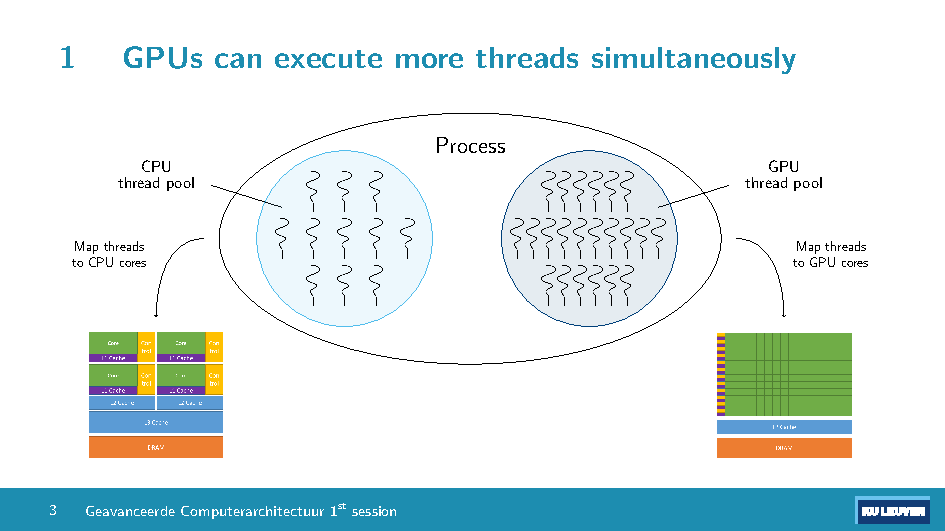
\includegraphics[width=0.72\linewidth, trim=0 20pt 0 0, clip, frame]{figures/slide-04.pdf}
\caption{GPUs can execute more threads simultaneously than CPUs.}
\end{figure}
\begin{figure}[H]
\centering
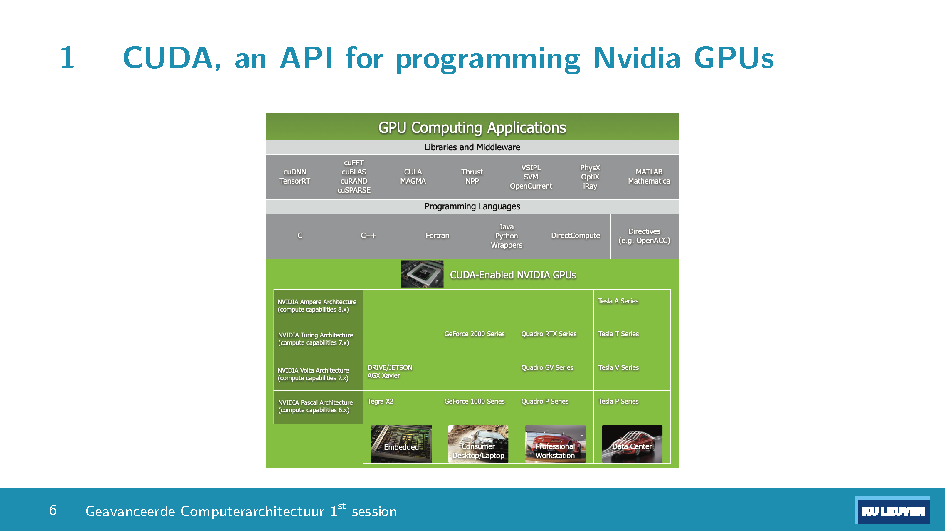
\includegraphics[width=0.72\linewidth, trim=0 20pt 0 0, clip, frame]{figures/slide-09.pdf}
\caption{CUDA, an API for programming NVIDIA GPUs.}
\end{figure}

\subsection{Lab sessions}

The below sections outline the six guided lab sessions (each 3h).

\textbf{Organization} --- 12 sessions in total:
\begin{itemize}[nosep]
  \item 5 lab sessions
  \item 7 project sessions (6 project, 1 presentations)
\end{itemize}

\subsection{Responsibilities and evaluation}

\begin{minipage}[t]{0.48\linewidth}
\textbf{Lab sessions: 50\%}
\begin{itemize}[nosep]
  \item 5 single-page reports, one per lab session
\end{itemize}
\end{minipage}\hfill
\begin{minipage}[t]{0.48\linewidth}
\textbf{Project: 50\%}
\begin{itemize}[nosep]
  \item Project report
  \item Project presentation
  \item Code release
\end{itemize}
\end{minipage}

%=====================================================================
\section{Project}

\subsection{Goal and organization}
\begin{itemize}
  \item The goal of the project is to tackle a computational challenge using the GPU.
  \item This should be something that aligns with your interests -- to support your thesis or another lab; to implement something for a hobby / private project; to boost your portfolio and get a better job.
  \item We will allocate 5 lab sessions to development and 1 session to the presentations.
\end{itemize}

\subsection{Implementation}
\begin{itemize}
  \item Use the concepts we have gotten acquainted with so far and feel free to explore other paradigms. You can use another programming language and also build on another library -- keep in mind that you should still understand and describe the intricacies of the implementation.
\end{itemize}

\subsection{Some topic examples}
In case you don't know where to start, here are a few biased examples:
\begin{itemize}
  \item An RF \textbf{ray tracer} to determine how Wi-Fi waves propagate in (and outside of) your kot.
  \item An \textbf{optimization algorithm} to determine where to put the Wi-Fi router for optimal coverage (considering either only yourself or all inhabitants).
  \item \textbf{Data compression} on an edge device that collects sensor samples and analyzes/compresses/transforms these in order to send the information over a low-throughput link.
  \item Real-time \textbf{statistical analysis} of a video stream.
\end{itemize}

\subsection{Grading -- guidelines based on thesis evaluation matrix}

\textbf{Implementation}
\begin{itemize}[nosep]
  \item The implementation works, while clearly addressing the tackled problem
  \item Includes the concepts introduced in the lab or sufficiently motivates other approaches
\end{itemize}

\textbf{Report} (no min/max length -- try to be concise)
\begin{itemize}[nosep]
  \item Clearly describes the problem and motivates the usage of the GPU
  \item Introduces the implementation and methods in detail (includes references to the repository or code listings)
  \item Highlights the shortcomings and possible improvements
\end{itemize}

\textbf{Presentation} (up to 10 min + 10 min for Q\&A)
\begin{itemize}[nosep]
  \item Clearly describes the problem and motivates the usage of the GPU
  \item Provides a high-level overview of the implementation
  \item Highlights the shortcomings and possible improvements
\end{itemize}

\subsection{Important dates}
Please submit the reports on time, so we can close off the lab on the day of the presentations (focus on the thesis / exams afterwards).

%=====================================================================
\section{Reading}

Read the first chapter of the CUDA Programming Guide:\\
\url{https://docs.nvidia.com/cuda/cuda-programming-guide/01-introduction/introduction.html}

With focus on:
\begin{itemize}[nosep]
  \item CUDA and the CUDA Programming Guide
  \item 1.1.1.\ The Graphics Processing Unit
  \item 1.1.2.\ The Benefits of Using GPUs
  \item 1.1.3.\ Getting Started Quickly
  \item 1.2.2.1.\ Thread Blocks and Grids
  \item 1.2.2.1.1.\ Thread Block Clusters
  \item 1.2.2.2.\ Warps and SIMT
  \item 1.2.3.4.\ Unified Memory
\end{itemize}

%=====================================================================
\section{Where to run?}
\begin{figure}[H]
\centering
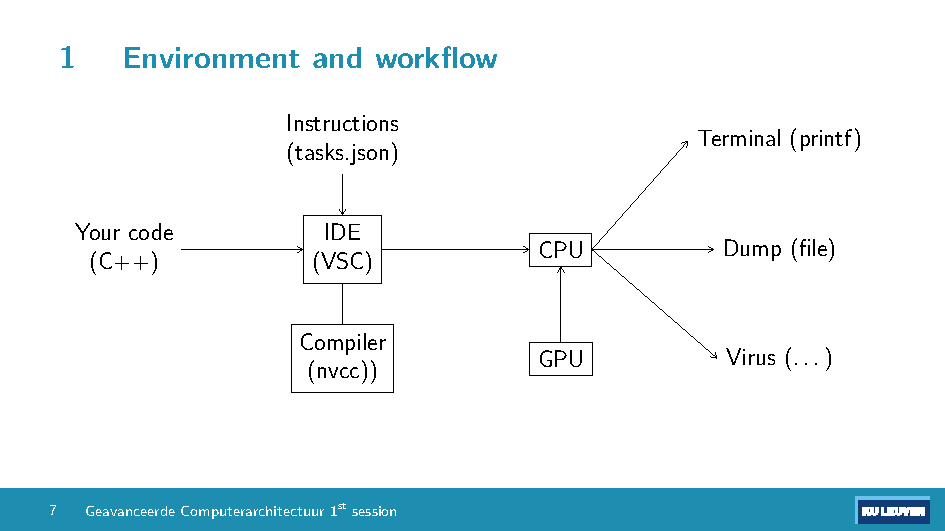
\includegraphics[width=0.72\linewidth, trim=0 20pt 0 0, clip, frame]{figures/slide-10.pdf}
\caption{Environment and workflow.}
\end{figure}

\subsection{On the lab PCs (no GPU of your own)}
\begin{enumerate}
  \item Use a desktop with a grey/silver front: these have an NVIDIA GPU (from next week).

  \begin{tabular}{@{}ll}
    GPU: & NVIDIA GeForce GT 730\\
    Compute capability: & 3.5\\
    Memory: & 1024 MB\\
    SMs: & 2 (192 cores per SM, 384 cores total)
  \end{tabular}
  \item Boot into Linux (not Windows).
  \item Log in:

  \begin{tabular}{@{}ll}
    user: & \texttt{student}\\
    password: & \texttt{studentXX} \quad (XX = the PC number)
  \end{tabular}

  Admin password (only if something needs to be changed): ask the teacher.
  \item Test:
\begin{lstlisting}[language=bash,numbers=none]
nvcc -arch=sm_35 -o hello hello.cu && ./hello
\end{lstlisting}
\end{enumerate}

\subsection{On your own laptop: Windows with WSL}
\begin{enumerate}
  \item Windows: check the laptop has an NVIDIA GPU, then install the latest NVIDIA driver from nvidia.com. Do \textbf{not} install any Linux driver inside WSL.
  \item PowerShell (admin):
\begin{lstlisting}[language=bash,numbers=none]
wsl --install
\end{lstlisting}
  Restart, open Ubuntu, create a user.
  \item Ubuntu:
\begin{lstlisting}[language=bash,numbers=none]
nvidia-smi
sudo apt update && sudo apt install -y build-essential
wget https://developer.download.nvidia.com/compute/cuda/repos/wsl-ubuntu/x86_64/cuda-keyring_1.1-1_all.deb
sudo dpkg -i cuda-keyring_1.1-1_all.deb
sudo apt update && sudo apt install -y cuda-toolkit
echo 'export PATH=/usr/local/cuda/bin:$PATH' >> ~/.bashrc && source ~/.bashrc
\end{lstlisting}
  \texttt{nvidia-smi} must show the GPU.\\
  GTX 10-series (Pascal) laptops: use \texttt{cuda-toolkit-12-9} instead of \texttt{cuda-toolkit}.
  \item VS Code: install on Windows + the ``WSL'' extension. Then in Ubuntu:
\begin{lstlisting}[language=bash,numbers=none]
mkdir ~/gca && cd ~/gca && code .
\end{lstlisting}
  Put the course \texttt{tasks.json} in \texttt{\textasciitilde/gca/.vscode/}
  \item Test:
\begin{lstlisting}[language=bash,numbers=none]
nvcc -o hello hello.cu && ./hello
\end{lstlisting}
\end{enumerate}

\subsection{On your own laptop: Linux (Ubuntu 24.04)}
\begin{enumerate}
  \item Driver:
\begin{lstlisting}[language=bash,numbers=none]
sudo ubuntu-drivers install
sudo reboot
nvidia-smi
\end{lstlisting}
  \texttt{nvidia-smi} must show the GPU. Top right it shows ``CUDA Version'': the newest CUDA this driver supports.
  \item Toolkit:
\begin{lstlisting}[language=bash,numbers=none]
sudo apt update && sudo apt install -y build-essential
wget https://developer.download.nvidia.com/compute/cuda/repos/ubuntu2404/x86_64/cuda-keyring_1.1-1_all.deb
sudo dpkg -i cuda-keyring_1.1-1_all.deb
sudo apt update && sudo apt install -y cuda-toolkit
echo 'export PATH=/usr/local/cuda/bin:$PATH' >> ~/.bashrc && source ~/.bashrc
\end{lstlisting}
  \begin{itemize}[nosep]
    \item Install only \texttt{cuda-toolkit} (not \texttt{cuda}: that also installs a second driver).
    \item The toolkit version (\texttt{nvcc --version}) must not be newer than the ``CUDA Version'' in \texttt{nvidia-smi}. If it is, or on GTX 10-series (Pascal) GPUs: use \texttt{cuda-toolkit-12-9} instead.
    \item Ubuntu 22.04: replace \texttt{ubuntu2404} with \texttt{ubuntu2204} in the \texttt{wget} line.
  \end{itemize}
  Simplest alternative (older CUDA 12.0, no PATH step needed):
\begin{lstlisting}[language=bash,numbers=none]
sudo apt install -y nvidia-cuda-toolkit
\end{lstlisting}
  \item VS Code:
\begin{lstlisting}[language=bash,numbers=none]
sudo snap install code --classic
mkdir ~/gca && cd ~/gca && code .
\end{lstlisting}
  Install the C/C++ extension. Put the course \texttt{tasks.json} in \texttt{\textasciitilde/gca/.vscode/}
  \item Test:
\begin{lstlisting}[language=bash,numbers=none]
nvcc -o hello hello.cu && ./hello
\end{lstlisting}
\end{enumerate}

%=====================================================================
\section{Examples: from ``hello'' to flipping an array}
\subsection{01\_hello.cu}
\begin{lstlisting}[language=CUDA]
// <cstdio> is the C standard input/output library (C++ name for stdio.h).
// We need it for printf on the CPU. On the GPU, CUDA provides printf itself.
#include <cstdio>

// __global__ marks a kernel: it is CALLED from the CPU but RUNS on the GPU.
// "global" because it is visible to both sides. The only way to run your own code
// on the GPU is through a kernel. Helpers marked __device__ can then be called from a kernel.
// void: -> A kernel MUST return void; results are written to memory.
__global__ void hello() {
    // this printf runs on the GPU and is NOT the stdio one. It has the same name and the buffer in GPU memory.
    printf("Hello from the GPU\n");
}

// main() ALWAYS runs on the CPU. Only the body of hello() runs on the GPU.
int main() {
    // Launch the kernel on the GPU: <<<number of blocks, threads per block>>>.
    // " launch the hello kernel with 1 block of 1 thread".
    // Each thread runs the whole body of hello() once, so 1 thread = 1 line of output.
    hello<<<1, 1>>>();
    // hello<<<2, 8>>>() would be 2 blocks of 8 threads = 16 threads which would be 16 times "Hello from the GPU".
    // The launch is asynchronous: the CPU does not wait and continues immediately.

    // cudaDeviceSynchronize() is a CUDA function, called on the CPU, that makes the CPU
    // wait until the GPU has finished all launched work. It also flushes the GPU's printf output.
    // Then the CPU simply continues with the next line, as it always would.
    // Without it, the program could end before the GPU has printed anything.
    // cudaDeviceSynchronize = wait for the GPU
    cudaDeviceSynchronize();


    // this is the normal C printf from <cstdio>, running on the CPU and writing to the terminal.
    printf("Hello from the CPU\n");
}

// Output:
// Hello from the GPU
// Hello from the CPU
\end{lstlisting}
\subsection{02\_threads.cu}
\begin{lstlisting}[language=CUDA]
#include <cstdio>

__global__ void hello() {
    // threadIdx.x is a built-in variable that exists automatically in every kernel.
    // It is the index of this thread within its block: 0..7 here.
    // Every thread sees a different value; that is how threads tell themselves apart.
    //
    // threads each run this line once, so you get 8 lines, 0 to 7.
    //
    // %d is a placeholder: printf replaces it with the integer argument (threadIdx.x).
    // \n is a newline.
    // (std::cout does not work on the GPU, only printf.)
    //
    // threadIdx is ONE variable, a struct with three fields: threadIdx.x, threadIdx.y, threadIdx.z.
    // (There is no "threadIdy"; it is always threadIdx.something.)
    // With a 1D launch like <<<1, 8>>>, only .x changes; .y and .z are always 0.
    printf("thread %d\n", threadIdx.x);
}

int main() {
    hello<<<1, 8>>>();
    cudaDeviceSynchronize();
}

// Output (order is not guaranteed, but within one block it is usually in order):
// thread 0
// thread 1
// thread 2
// thread 3
// thread 4
// thread 5
// thread 6
// thread 7
//
// Why not guaranteed: all threads run in parallel, and the GPU's hardware scheduler decides
// which threads execute when. Threads are run in groups of 32 (warps). Within one warp the
// printf usually comes out in thread order, but CUDA does not promise it. Between warps and
// between blocks there is no order at all: blocks can run on different parts of the GPU, at the
// same time, in any order. 
// never write code that depends on thread order!
\end{lstlisting}
\begin{figure}[H]
\centering
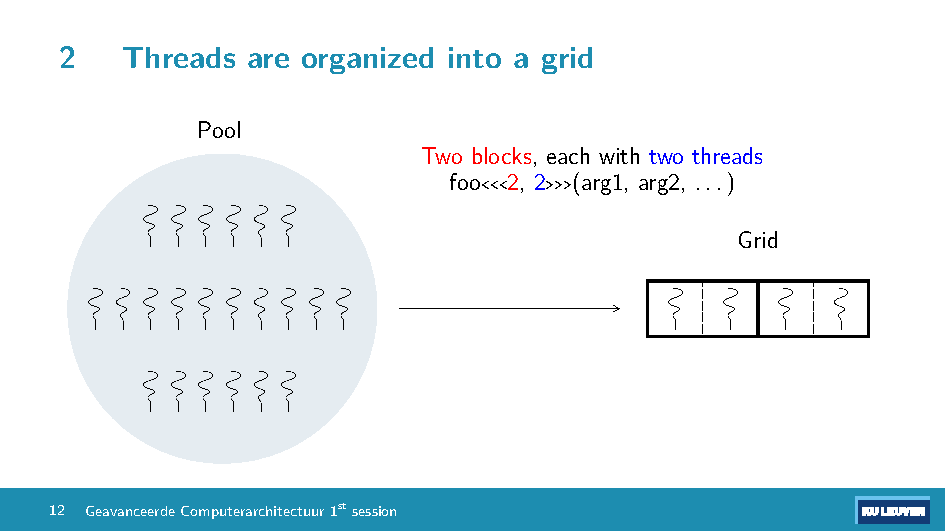
\includegraphics[width=0.72\linewidth, trim=0 20pt 0 0, clip, frame]{figures/slide-15.pdf}
\caption{Threads are organized into a grid of blocks.}
\end{figure}
\subsection{02b\_threads\_2d.cu}
\begin{lstlisting}[language=CUDA]
// Why 2D/3D? It is purely a convenience for the programmer, not a hardware feature.
// The hardware still sees the threads as one long line (x counts fastest, then y, then z)
// and groups them into warps of 32 in that order. Performance is the same.
// The benefit: the indices match the shape of the data.
//   - 2D: images (x = column, y = row), matrices.  3D: volumes (CT scans, voxels, 3D simulations).
//   - Without it you would compute row = i / W and col = i % W yourself; with 2D you get them directly.
// Very common: almost every image or matrix kernel uses 2D blocks, e.g. 16 x 16 threads.
// Every CUDA GPU supports 1D, 2D and 3D blocks and grids (block z is limited to 64).
#include <cstdio>

__global__ void hello() {
    // Now the block is 2D, so every thread has two indices:
    //   threadIdx.x = column inside the block: 0..3
    //   threadIdx.y = row inside the block:    0..1
    printf("thread x=%d y=%d\n", threadIdx.x, threadIdx.y);
}

int main() {
    // dim3 is a CUDA type with three numbers (x, y, z); missing ones default to 1.
    // dim3 threads(4, 2) = a block of 4 columns by 2 rows = 8 threads.
    // Writing <<<1, 8>>> is shorthand for dim3(1, 1, 1) blocks and dim3(8, 1, 1) threads.
    // The grid can be 2D in the same way: dim3 blocks(2, 3) gives blockIdx.x and blockIdx.y.
    // 2D is convenient for images and matrices: x = column, y = row.
    // dim3 is a CUDA TYPE: a small struct with three numbers x, y, z (like int, but with three values).
    // "threads"is just the name of our variable; 
    // The built-ins are only threadIdx, blockIdx, blockDim and gridDim.
    dim3 threads(4, 2);
    hello<<<1, threads>>>();
    cudaDeviceSynchronize();
}

// Output (same 8 threads as 02, but now each has an x and a y; order not guaranteed):
// thread x=0 y=0
// thread x=1 y=0
// thread x=2 y=0
// thread x=3 y=0
// thread x=0 y=1
// thread x=1 y=1
// thread x=2 y=1
// thread x=3 y=1
\end{lstlisting}
\subsection{03\_blocks.cu}
\begin{lstlisting}[language=CUDA]
#include <cstdio>

__global__ void hello() {
    // Also built-in variables:
    // blockIdx.x = index of this block in the grid: 0..1 here
    // blockDim.x = threads per block, i.e. the 2nd launch number: 4 here
    // gridDim.x  = number of blocks, i.e. the 1st launch number: 2 here
    //
    // to get a unique global index: block 1, thread 2 -> 1*4+2 = 6.
    // global index = blockIdx.x * blockDim.x + threadIdx.x 
    //
    // Block 0 covers indices 0..3, so block 1 starts after those 4: at index 4.
    int i = blockIdx.x * blockDim.x + threadIdx.x;  
    printf("block %d thread %d -> global index %d\n", blockIdx.x, threadIdx.x, i);
}

int main() {
    hello<<<2, 4>>>();
    cudaDeviceSynchronize();
}

// Output (block 1 may print before block 0; that differs between runs):
// block 0 thread 0 -> global index 0
// block 0 thread 1 -> global index 1
// block 0 thread 2 -> global index 2
// block 0 thread 3 -> global index 3
// block 1 thread 0 -> global index 4
// block 1 thread 1 -> global index 5  
// block 1 thread 2 -> global index 6
// block 1 thread 3 -> global index 7  e.g. (1 * 4) + 3
\end{lstlisting}
\begin{figure}[H]
\centering
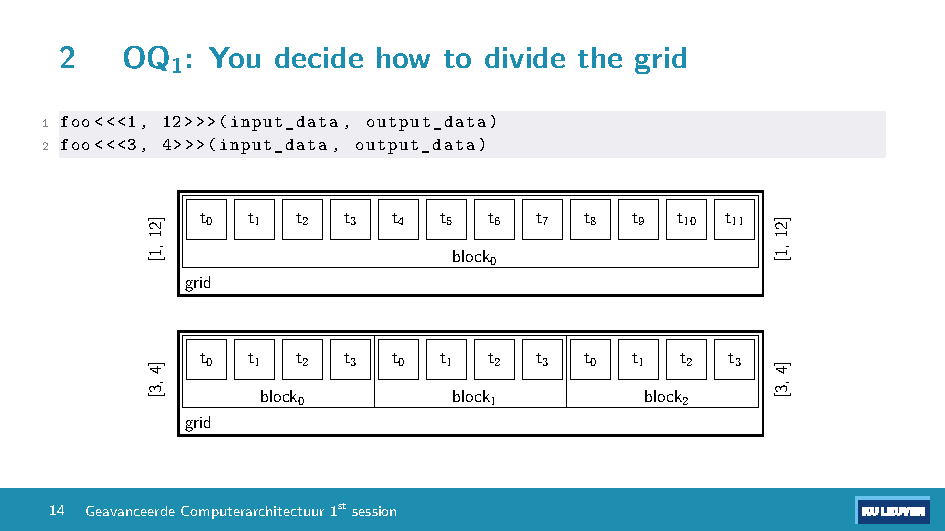
\includegraphics[width=0.72\linewidth, trim=0 20pt 0 0, clip, frame]{figures/slide-17.pdf}
\caption{You decide how to divide the grid.}
\end{figure}
\begin{figure}[H]
\centering
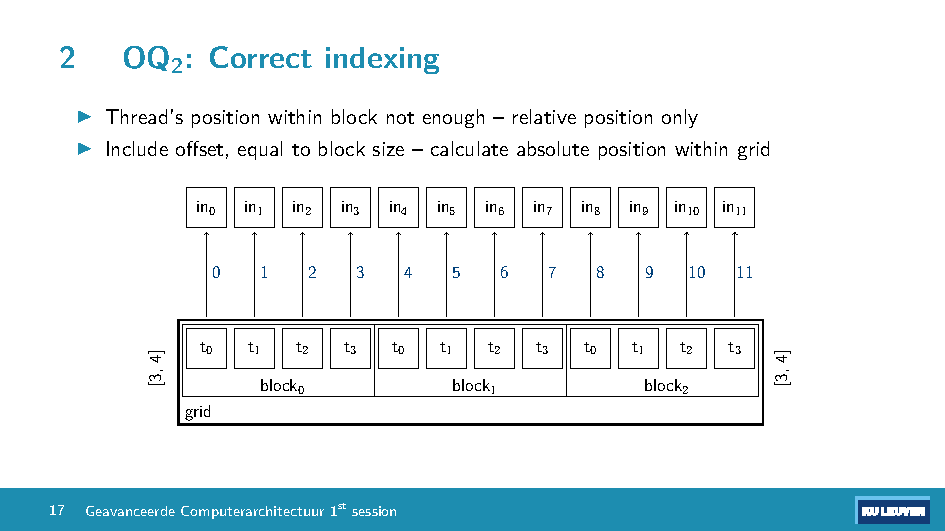
\includegraphics[width=0.72\linewidth, trim=0 20pt 0 0, clip, frame]{figures/slide-20.pdf}
\caption{Correct indexing: add the block offset to get the absolute position.}
\end{figure}
\subsection{04\_memory.cu}
\begin{lstlisting}[language=CUDA]
//  Every line in main() runs on the CPU; only the kernel fill() runs on the GPU.
//   1. int* a;                                   (CPU) Create an empty pointer. It points nowhere yet.
//   2. cudaMallocManaged(&a, N * sizeof(int));   (CPU calls it) Reserve 32 bytes that both CPU and GPU
//                                                can reach, and put the address into a. The memory
//                                                exists now, but holds no useful values yet.
//   3. fill<<<2, 4>>>(a);                        (CPU starts it, GPU runs it) 8 GPU threads each write
//                                                their own index into their own element: 0 1 2 ... 7.
//                                                The CPU does not wait here.
//   4. cudaDeviceSynchronize();                  (CPU) Wait until the GPU has finished filling.
//   5. for loop with printf                      (CPU) Read the array and print 0 1 2 3 4 5 6 7.
//   6. cudaFree(a);                              (CPU calls it) Give the memory back; we are done with it.
#include <cstdio>

// Preprocessor constant: before compiling, every N in the file is replaced by 8.
// It represents the length of the array.
#define N 8

// A kernel that receives a pointer adress to the array.
// It does not MAKE the array: the memory is reserved in main() by cudaMallocManaged.
// This kernel FILLS the existing array: it writes the values 0..7 into it.
//
// This replaces the CPU loop "for (i = 0; i < N; i++) a[i] = i;" — the threads ARE the loop.
__global__ void fill(int* a) {
    int i = blockIdx.x * blockDim.x + threadIdx.x;
    // No bounds check needed HERE because N = 8 and we launch exactly 2 * 4 = 8 threads:
    a[i] = i;
}

int main() {
    // a is a pointer: a variable that holds a memory address (the start of an int array).
    // It does not point anywhere yet.
    int* a;

    // Allocate N * sizeof(int) = 8 * 4 = 32 bytes of unified memory, (a property of int is that they use 4 bytes)
    // reachable by both the CPU and the GPU.
    // &a is the address of the pointer itself, so the function can write the new address into a.
    cudaMallocManaged(&a, N * sizeof(int));   

    fill<<<2, 4>>>(a);

    // The CPU waits until the kernel is done. Only then is it safe to read a on the CPU.
    cudaDeviceSynchronize();

    for (int i = 0; i < N; i++) printf("%d ", a[i]);   
    printf("\n");

    // Release the memory from cudaMallocManaged (the CUDA equivalent of free()).
    cudaFree(a);
}

// Output:
// 0 1 2 3 4 5 6 7
\end{lstlisting}
\paragraph{Why we need bounds.} The number of threads you launch is always blocks $\times$ threads per block, so it's always a multiple of the block size. The size of your data (N) is set by the problem and almost never matches. The bounds check \texttt{if (i < N)} stops the extra threads from reading or writing memory outside the array. Without it, the program can silently corrupt memory or crash, even when the output looks correct.
\begin{figure}[H]
\centering
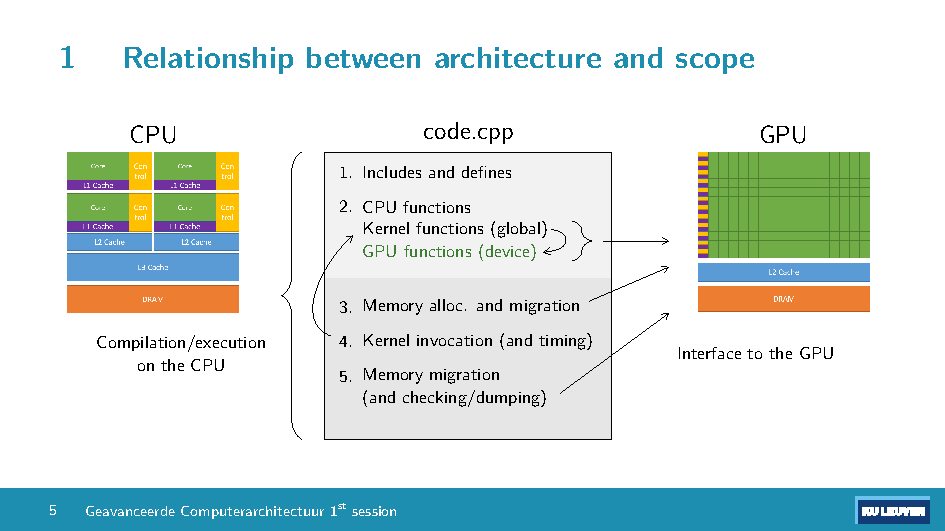
\includegraphics[width=0.72\linewidth, trim=0 20pt 0 0, clip, frame]{figures/slide-08.pdf}
\caption{Which part of the program runs on the CPU and which on the GPU.}
\end{figure}
\newpage
\subsection{05\_bounds.cu}
\begin{lstlisting}[language=CUDA]
#include <cstdio>

#define N 10

__global__ void fill(int* a, int n) {
    int i = blockIdx.x * blockDim.x + threadIdx.x;
    // We launch 3 blocks * 4 threads = 12 threads, but the array has only 10 elements.
    // Threads 10 and 11 must do nothing, otherwise they write outside the array.
    if (i < n) a[i] = i;
}

int main() {
    int* a;
    cudaMallocManaged(&a, N * sizeof(int));

    int threads = 4;
    // Integer division rounds DOWN: 10 / 4 = 2 blocks = 8 threads, which is too few.
    // Adding (threads - 1) makes it round UP: (10 + 3) / 4 = 3 blocks = 12 threads.
    int blocks = (N + threads - 1) / threads;

    // N is the #define above (10). We pass it to the kernel as parameter n,
    // because the kernel needs the array length for its bounds check.
    fill<<<blocks, threads>>>(a, N);
    cudaDeviceSynchronize();

    for (int i = 0; i < N; i++) printf("%d ", a[i]);
    printf("\n");

    cudaFree(a);
}

// Output (threads 10 and 11 exist but write nothing):
// 0 1 2 3 4 5 6 7 8 9
\end{lstlisting}
\subsection{06\_flip.cu}
\begin{lstlisting}[language=CUDA]
// The plan: the CPU makes two arrays and fills "in" with 0 1 2 ... 8.
// The GPU copies every element of "in" to its mirrored position in "out".
// The CPU then prints both arrays and checks the result.
//
// Steps in main():
//   1. Reserve two arrays of 9 ints: in and out.
//   2. Fill in on the CPU with 0 ... 8.
//   3. Choose the launch: 4 threads per block, (9 + 3) / 4 = 3 blocks = 12 threads.
//   4. Launch flip: threads 0..8 each move one element; threads 9..11 are stopped by the bounds check.
//   5. Wait for the GPU.
//   6. Print in and out on the CPU.
//   7. Verify: in[i] was i, so out[i] must be N - 1 - i.
//   8. Free both arrays.
//
// About step 3 — warps:
//   The GPU never runs a single thread on its own. It runs threads in groups of 32, called a warp.
//   All 32 threads of a warp execute the same instruction at the same time.
//   Every block is cut into warps:
//     block of 4 threads   -> 1 warp, of which only 4 lanes work and 28 sit idle
//     block of 256 threads -> 8 full warps, nothing wasted
//   So in real code the block size is a multiple of 32 (typically 256).
//   Here we use 4 only to keep the example and its output small.
//
//   Real code example, for one million elements:
//     #define N 1000000
//     int threads = 256;
//     int blocks = (N + threads - 1) / threads;   -> 3907 blocks
//   3907 * 256 = 1,000,192 threads; the last 192 are stopped by the bounds check.
//   (With N that large you would not print the arrays; the verification loop does the checking.)
//
// Why two arrays: every thread reads from one array and writes to another, so no thread can
// overwrite a value that another thread still needs. The order in which threads run does not matter.

#include <cstdio>

#define N 9

// in  = pointer to the input array (0 1 2 ... 8). const = the kernel promises to only read it.
// out = pointer to the output array; the kernel writes the flipped values here.
// n   = number of elements (9), needed for the mirror position and the bounds check.
__global__ void flip(const int* in, int* out, int n) {
    int i = blockIdx.x * blockDim.x + threadIdx.x;
    // this is the flipping logic: each thread puts its element at the mirrored position.
    if (i < n) out[n - 1 - i] = in[i];
}

int main() {
    int *in, *out;
    cudaMallocManaged(&in, N * sizeof(int));
    cudaMallocManaged(&out, N * sizeof(int));

    // The starting array is made here: the cudaMallocManaged above reserves the memory,
    // and this loop fills it on the CPU with 0 1 2 ... 8.
    for (int i = 0; i < N; i++) in[i] = i;

    int threads = 4;    
    int blocks = (N + threads - 1) / threads; //3
    flip<<<blocks, threads>>>(in, out, N);
    cudaDeviceSynchronize();

    printf("in:  ");
    for (int i = 0; i < N; i++) printf("%d ", in[i]);
    printf("\nout: ");
    for (int i = 0; i < N; i++) printf("%d ", out[i]);
    printf("\n");

    // check
    for (int i = 0; i < N; i++) {
        if (out[i] != N - 1 - i) {
            printf("error at %d\n", i);
            return 1;
        }
    }
    printf("correct\n");

    cudaFree(in);
    cudaFree(out);
}

// Output:
// in:  0 1 2 3 4 5 6 7 8
// out: 8 7 6 5 4 3 2 1 0
// correct
\end{lstlisting}
\begin{figure}[H]
\centering
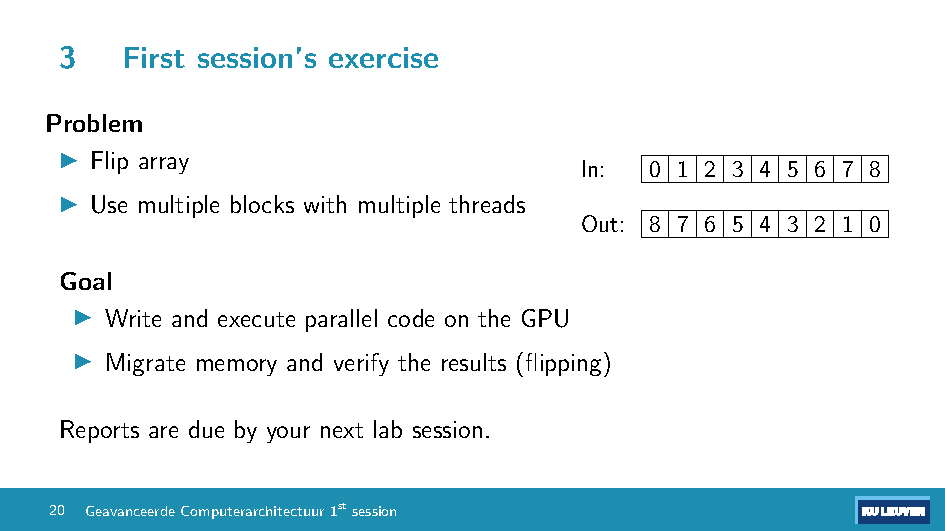
\includegraphics[width=0.72\linewidth, trim=0 20pt 0 0, clip, frame]{figures/slide-23.pdf}
\caption{First session's exercise: flip an array.}
\end{figure}
\newpage
\subsection{07\_flip\_inplace.cu}
\begin{lstlisting}[language=CUDA]
// In-place is an alternative with one advantage and some drawbacks:
//   + Uses ONE array instead of two: half the memory.
//   - Not faster: both versions read N values and write N values in total.
//   - Easier to get wrong: if all N threads simply copy their element to the mirror position,
//     a thread can overwrite a value that another thread has not read yet (a race condition,
//     topic of session 2). That is why only the first half of the threads work, each swapping one pair.
//   - The original input is gone afterwards, so you cannot compare against it.
// It is included mainly to show a race-condition trap.
//
// What is a race condition?
//   Two or more threads access the SAME memory location, at least one of them WRITES,
//   and nothing controls which one goes first. The result then depends on timing: on which
//   thread happens to be faster. It can be right in one run and wrong in the next.
//   On a GPU, thousands of threads run in parallel in no guaranteed order, so this is easy to cause.
//   Analogy: two people withdraw money from the same account at the same moment. Both read
//   balance 100, both subtract 50, both write back 50. One withdrawal is lost.
//   How to avoid it:
//     - make sure every memory location is written by only one thread (as in 06 and the swap below)
//     - or use synchronization / atomic operations (session 2).
//
// The race condition, concretely. The "obvious" in-place kernel would be:
//
//     if (i < n) a[n - 1 - i] = a[i];      // WRONG: all 9 threads, one array
//
// Thread 0 must write a[0] (= 0) into a[8]. Thread 8 must write a[8] (= 8) into a[0].
// Both touch a[0] and a[8], and nobody decides who goes first:
//   - if thread 8 reads a[8] BEFORE thread 0 overwrites it: a[0] = 8   (correct)
//   - if thread 8 reads a[8] AFTER  thread 0 overwrote it:  a[0] = 0   (wrong: the 8 is lost)
// The same happens for every pair. A possible result is 0 1 2 3 4 3 2 1 0 (a mirror, not a flip),
// and it can differ from run to run. That is what a race condition is: the result depends on
// which thread happens to be faster.
//
// The fix below: only n / 2 threads, and each thread does the WHOLE swap of one pair itself.
// Pair (i, n-1-i) is touched by exactly one thread, so no two threads ever touch the same element.
// tmp is a local variable: every thread has its own private copy (in its own register).

#include <cstdio>

#define N 9

__global__ void flip(int* a, int n) {
    int i = blockIdx.x * blockDim.x + threadIdx.x;
    if (i < n / 2) {
        int tmp = a[i];
        a[i] = a[n - 1 - i];
        a[n - 1 - i] = tmp;
    }
}

int main() {
    int* a;
    cudaMallocManaged(&a, N * sizeof(int));

    for (int i = 0; i < N; i++) a[i] = i;

    int threads = 4;
    int blocks = (N / 2 + threads - 1) / threads;
    flip<<<blocks, threads>>>(a, N);
    cudaDeviceSynchronize();

    for (int i = 0; i < N; i++) printf("%d ", a[i]);
    printf("\n");

    cudaFree(a);
}

// Launch: N / 2 = 4 pairs -> (4 + 3) / 4 = 1 block of 4 threads.
// Thread 0 swaps 0<->8, thread 1 swaps 1<->7, thread 2 swaps 2<->6, thread 3 swaps 3<->5.
// The middle element (4) stays where it is.
// Output:
// 8 7 6 5 4 3 2 1 0
\end{lstlisting}

%=====================================================================
\section{Expected for next week}

A \LaTeX-created PDF document with a solution for exercise \texttt{08\_flip\_2d.cu}.

\subsection{08\_flip\_2d.cu: flip a 2D array (mirror an image horizontally)}

\textbf{Problem.} A 2D array of W columns by H rows (think: an image). Reverse every row:

\begin{center}
\begin{tabular}{cc}
\texttt{in:} & \texttt{out:}\\
\begin{tabular}{rrrrrr} 0&1&2&3&4&5\\ 6&7&8&9&10&11 \end{tabular} &
\begin{tabular}{rrrrrr} 5&4&3&2&1&0\\ 11&10&9&8&7&6 \end{tabular}
\end{tabular}
\end{center}

Use a 2D grid of 2D blocks: every thread handles one element and gets an \texttt{x} (column) and a \texttt{y} (row).

\textbf{Goal.}
\begin{itemize}[nosep]
  \item Compute \texttt{x} and \texttt{y} for each thread.
  \item Convert \texttt{(x, y)} to a position in memory.
  \item Bounds check in \textbf{both} directions.
  \item Verify the result on the CPU.
\end{itemize}

%=====================================================================
\newpage
\section{Cheat sheet}

This section lists several functions, definitions, etc., handy for the GCA lab. It is a living document, where updates are added according to the lab sessions and feedback from the students. Thanks for pointing things out.

\textbf{GPU memory allocation}
\begin{lstlisting}[language=CUDA,numbers=none]
float* d_A;
cudaMalloc(&d_A, size);
\end{lstlisting}

\textbf{Memory migration to / from GPU}
\begin{lstlisting}[language=CUDA,numbers=none]
float* h_A = (float*)malloc(size);
cudaMemcpy(d_A, h_A, size, cudaMemcpyHostToDevice);
cudaMemcpy(h_A, d_A, size, cudaMemcpyDeviceToHost);
\end{lstlisting}

\textbf{Kernel invocation (100 blocks, with 80 threads each)}
\begin{lstlisting}[language=CUDA,numbers=none]
foo<<<100, 80>>>(d_A);
\end{lstlisting}

\textbf{Thread indexing}
\begin{lstlisting}[language=CUDA,numbers=none]
int i = threadIdx.x;
\end{lstlisting}

\textbf{Setting to global scope (invoked by CPU or GPU)}
\begin{lstlisting}[language=CUDA,numbers=none]
__global__ void foo(d_A){...}
\end{lstlisting}

\textbf{Setting to GPU scope (invoked by GPU)}
\begin{lstlisting}[language=CUDA,numbers=none]
__device__ float foo(d_A){...}
\end{lstlisting}

\textbf{Timing (CPU)}
\begin{lstlisting}[language=CUDA,numbers=none]
#include <chrono>
const auto start = std::chrono::steady_clock::now();
...
const auto end = std::chrono::steady_clock::now();
const std::chrono::duration<double> elapsed_seconds{end - start};
\end{lstlisting}

\textbf{Timing (GPU)}
\begin{lstlisting}[language=CUDA,numbers=none]
cudaEvent_t start, stop;
cudaEventCreate(&start);
cudaEventCreate(&stop);
cudaEventRecord(start);
...
cudaEventSynchronize();
cudaEventRecord(stop);
float milliseconds;
cudaEventElapsedTime(&milliseconds, start_cuda, stop_cuda);
\end{lstlisting}

\end{document}
